% Attended-speaker decoding section -- compiles standalone but is styled as a
% mid-paper journal section (section counter starts at 4; no title/abstract).
% Build: latexmk -pdf attended_speaker_decoding.tex   (or pdflatex x2)
\documentclass[10pt,twocolumn]{article}
\usepackage[T1]{fontenc}
\usepackage{lmodern}
\usepackage[letterpaper,margin=0.85in,columnsep=0.28in]{geometry}
\usepackage{amsmath,amssymb}
\usepackage{booktabs}
\usepackage{array}
\usepackage{graphicx}
\usepackage{siunitx}
\usepackage{microtype}
\usepackage{xcolor}
\usepackage[hidelinks]{hyperref}
\usepackage{caption}
\usepackage{subcaption}
\usepackage{float}      % [H] = put the float exactly here, no drifting
\usepackage{placeins}  % \FloatBarrier confines floats to their section
\usepackage{tikz}
\usetikzlibrary{positioning,arrows.meta,fit,backgrounds,calc,shadows}
\captionsetup{font=small,labelfont=bf}
\graphicspath{{figs/}}

% ---- shared, professional figure style (one visual language) ----------------
\definecolor{cInp}{HTML}{E8EFFB}\definecolor{cInpB}{HTML}{6F9BD8}
\definecolor{cBr}{HTML}{FFFFFF}\definecolor{cBrB}{HTML}{8A94A6}
\definecolor{cCon}{HTML}{EAF1FB}\definecolor{cConB}{HTML}{3F6FB5}
\definecolor{cSpa}{HTML}{E7F4F1}\definecolor{cSpaB}{HTML}{2E8B83}
\definecolor{cFrz}{HTML}{F0E9F7}\definecolor{cFrzB}{HTML}{8E6FB0}
\definecolor{cEmb}{HTML}{E4F3F6}\definecolor{cEmbB}{HTML}{4F9DAE}
\definecolor{cFus}{HTML}{FCEEDD}\definecolor{cFusB}{HTML}{D98A33}
\definecolor{cOut}{HTML}{E6F5E6}\definecolor{cOutB}{HTML}{4F9D52}
\tikzset{
  >=Stealth,
  nd/.style={draw,rounded corners=2.5pt,align=center,line width=0.7pt,
             drop shadow={shadow xshift=0.5pt,shadow yshift=-0.7pt,fill=black,opacity=0.16}},
  inp/.style ={nd,fill=cInp,draw=cInpB},
  brn/.style ={nd,fill=cBr ,draw=cBrB},
  frz/.style ={nd,fill=cFrz,draw=cFrzB},
  emb/.style ={nd,fill=cEmb,draw=cEmbB},
  vbr/.style ={nd,fill=cSpa,draw=cSpaB},
  fuse/.style={nd,fill=cFus,draw=cFusB},
  outn/.style={nd,fill=cOut,draw=cOutB},
  proc/.style={nd,fill=gray!8,draw=cBrB},
  ghost/.style={draw=gray!55,dashed,rounded corners=2.5pt,align=center,fill=gray!6,text=gray!55},
  grp/.style={thick,dashed,rounded corners=3pt},
  flow/.style ={->,line width=0.8pt,gray!55!black},
  flowd/.style={->,line width=0.8pt,dashed,gray!70},
}
\renewcommand{\arraystretch}{1.18}
\sisetup{detect-weight=true,mode=text}
\newcommand{\ttt}[1]{\texttt{\small #1}}

% ---- result macros (single source of truth) --------------------------------
% Latest run = job 6056844 (audio-window-trimmed V-JEPA cache, content/orienting split).
% Within-subject 5-fold, chance 0.25
\newcommand{\intraEnv}{0.428}\newcommand{\intraEnvS}{0.095}
\newcommand{\intraSpec}{0.418}\newcommand{\intraSpecS}{0.077}
\newcommand{\intraSem}{0.345}\newcommand{\intraSemS}{0.096}
\newcommand{\intraDirLda}{0.555}\newcommand{\intraDirLdaS}{0.231}
% gaze-MLP head comparison (regularisation lever)
\newcommand{\intraDirMlp}{0.527}\newcommand{\intraDirMlpS}{0.215}
\newcommand{\intraMlpAvg}{0.563}\newcommand{\intraMlpAvgS}{0.167}
\newcommand{\intraMlpRel}{0.565}\newcommand{\intraMlpRelS}{0.185}
\newcommand{\intraMlpStack}{0.503}\newcommand{\intraMlpStackS}{0.184}
% LDA-head fusion, no video
\newcommand{\intraLdaRel}{0.614}\newcommand{\intraLdaRelS}{0.205}
\newcommand{\intraLdaRelv}{0.616}\newcommand{\intraLdaRelvS}{0.201}
% honest content-only / orienting partial fusions (no video)
\newcommand{\cfusedI}{0.440}\newcommand{\cfusedIS}{0.098}
\newcommand{\sfusedI}{0.547}\newcommand{\sfusedIS}{0.240}
% vision branch: fovea-only (headline) vs scene+fovea
\newcommand{\visFov}{0.662}\newcommand{\visFovS}{0.220}
\newcommand{\visSF}{0.649}\newcommand{\visSFS}{0.229}
\newcommand{\visWeight}{0.384}
% orienting fusion + video, and full fused + video
\newcommand{\sfusedVid}{0.667}\newcommand{\sfusedVidS}{0.225}
\newcommand{\fusedSF}{0.681}\newcommand{\fusedSFS}{0.218}
\newcommand{\fusedFovRel}{0.695}\newcommand{\fusedFovRelS}{0.202}
\newcommand{\fusedFovRelv}{0.700}\newcommand{\fusedFovRelvS}{0.207}
% MS+recon encoder control + VALIGN content ablation (within)
\newcommand{\msrEnv}{0.306}\newcommand{\msrSpec}{0.315}\newcommand{\msrSem}{0.268}
\newcommand{\valEnv}{0.296}\newcommand{\valSpec}{0.318}\newcommand{\valSem}{0.276}   % scene target
\newcommand{\valfEnv}{0.295}\newcommand{\valfSpec}{0.310}\newcommand{\valfSem}{0.277}% fovea target
\newcommand{\cfusedVal}{0.313}\newcommand{\cfusedValS}{0.075}
\newcommand{\fusedFovVal}{0.674}\newcommand{\fusedFovValS}{0.219}
% Null (input-shuffle), within
\newcommand{\nullFused}{0.250}\newcommand{\nullFusedS}{0.038}
\newcommand{\nullCfused}{0.248}\newcommand{\nullCfusedS}{0.028}
\newcommand{\nullSfused}{0.252}\newcommand{\nullSfusedS}{0.030}
\newcommand{\nullVis}{0.271}\newcommand{\nullVisS}{0.052}
% LOSO (job 6056844, fovea-only), chance 0.25
\newcommand{\losoEnv}{0.358}\newcommand{\losoEnvS}{0.045}
\newcommand{\losoSpec}{0.353}\newcommand{\losoSpecS}{0.071}
\newcommand{\losoSem}{0.360}\newcommand{\losoSemS}{0.073}
\newcommand{\losoDirLda}{0.540}\newcommand{\losoDirLdaS}{0.211}
\newcommand{\losoVisFov}{0.592}\newcommand{\losoVisFovS}{0.156}
\newcommand{\losoCfused}{0.398}\newcommand{\losoCfusedS}{0.068}
\newcommand{\losoSfusedVid}{0.641}\newcommand{\losoSfusedVidS}{0.181}
\newcommand{\losoFusedVid}{0.642}\newcommand{\losoFusedVidS}{0.173}
\newcommand{\losoLdaRel}{0.520}\newcommand{\losoLdaRelS}{0.136}   % no-video LOSO baseline (job 6138857)
\newcommand{\losoDirMlp}{0.494}\newcommand{\losoDirMlpS}{0.166}   % gaze-MLP LOSO (job 6138857)
\newcommand{\losoVisSF}{0.607}\newcommand{\losoVisSFS}{0.199}     % video scene+fovea LOSO
\newcommand{\losoSfusedGaze}{0.540}\newcommand{\losoSfusedGazeS}{0.211} % orienting, gaze only (no video)
\newcommand{\losoFusedRelv}{0.644}\newcommand{\losoFusedRelvS}{0.161}   % full +video, relv (best LOSO)
\newcommand{\nullLosoFused}{0.270}\newcommand{\nullLosoFusedS}{0.038}
\newcommand{\losoNullCfused}{0.275}\newcommand{\losoNullCfusedS}{0.038}
% format helpers
\newcommand{\pmv}[2]{$#1\!\pm\!#2$}
\newcommand{\acc}[2]{$#1$\,{\footnotesize$\pm#2$}}   % right-aligned mean +- sd

\setcounter{section}{3}      % render as Section 4 (mid-paper)
\setcounter{table}{0}
\setcounter{figure}{0}
\setcounter{equation}{0}

\begin{document}
\pagestyle{empty}

\section{Attended-Speaker Decoding}
\label{sec:asd}

A listener sits in a room and attends one of several talkers playing
simultaneously from fixed loudspeakers. Our goal is to recover \emph{which}
talker, from the signals we record while they listen. Each $\approx\!35$\,s trial
plays four attendable talkers (loudspeakers $1$--$4$) plus two distractors
(loudspeakers $5$--$6$) that are never the target; the decoding task is thus a
four-way choice (chance $=0.25$), with $100$ trials per subject. We have four
recorded signals to work with (Fig.~\ref{fig:inputs}): scalp \textbf{EEG}, the
per-talker \textbf{audio}, the listener's \textbf{gaze}, and an egocentric
\textbf{scene video} from the eye-tracking glasses.

\begin{figure}[t]
\centering
\setlength{\tabcolsep}{1.5pt}
\begin{tabular}{cc}
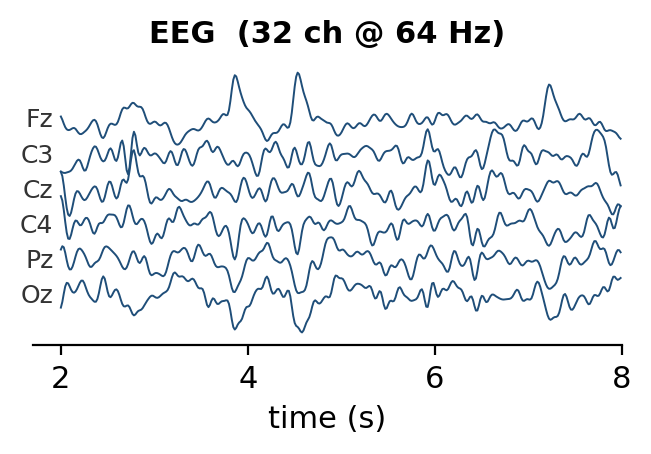
\includegraphics[width=0.475\columnwidth]{ico_eeg.png} &
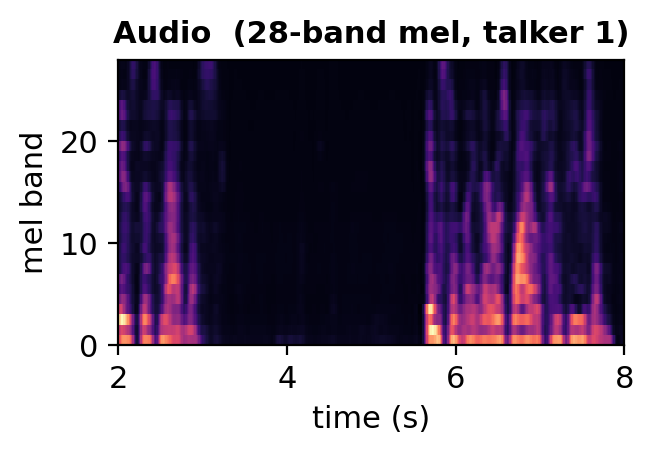
\includegraphics[width=0.475\columnwidth]{ico_audio.png} \\[1pt]
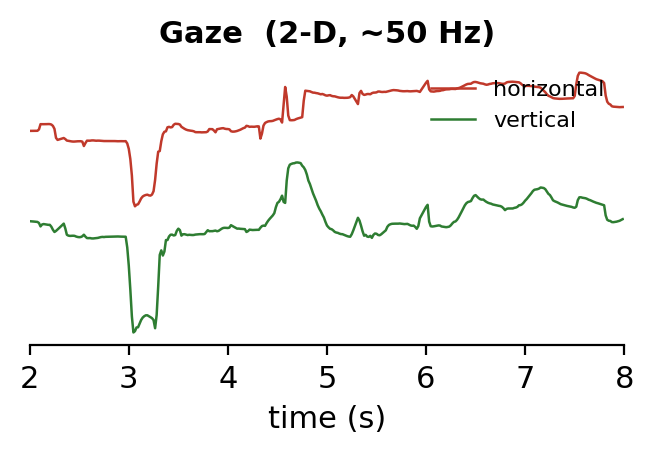
\includegraphics[width=0.475\columnwidth]{ico_gaze.png} &
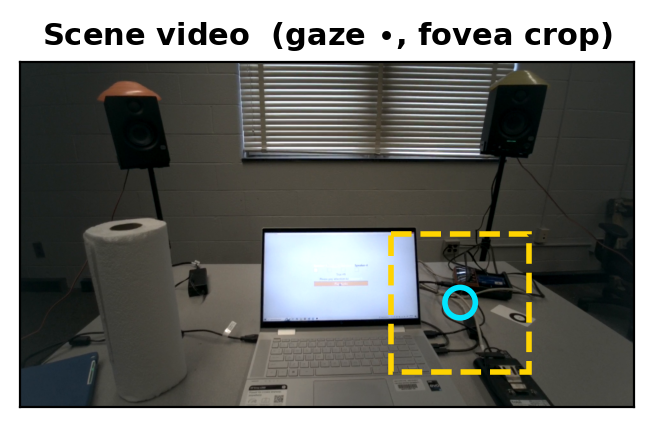
\includegraphics[width=0.475\columnwidth]{ico_scene.png} \\
\end{tabular}
\caption{\textbf{The four input signals} (one example trial). \emph{EEG}: $32$
scalp channels of brain activity. \emph{Audio}: each talker's speech as a
$28$-band mel spectrogram (one shown). \emph{Gaze}: the listener's eye position
over time. \emph{Scene video}: the egocentric view---note it shows
\emph{loudspeakers, not faces}, so there is no lip motion to read; the only thing
it adds is \emph{where} the listener looks (cyan dot), from which we crop a
foveal patch (yellow). These motivate the modelling choices throughout.}
\label{fig:inputs}
\end{figure}

\paragraph{Why a branch-and-fuse design.}
These signals are wildly unequal as attention cues. The brain's tracking of the
attended speech is real but \emph{faint}; gaze, by contrast, is a \emph{strong}
cue, because in a free-field room listeners tend to look toward whom they attend.
If we poured all signals into one network, training would be dominated by the
strong cue and the weak one would simply be overfit, and we could never say which
signal actually carried the decision. We therefore train one small,
\emph{single-cue} model per signal (a ``branch''), freeze it, and combine the
branches' class probabilities with a lightweight late fusion
(Fig.~\ref{fig:arch}). This keeps each cue interpretable, lets a
reliability-aware combiner trust strong cues over weak ones, and lets us add or
remove a cue---such as the video of Section~\ref{sec:asd-video}---without
disturbing the rest. The branches group naturally into two families:
\emph{content} branches that decode \emph{what} is being said, and \emph{spatial}
branches that decode \emph{where} attention points.

\begin{figure*}[t]
\centering
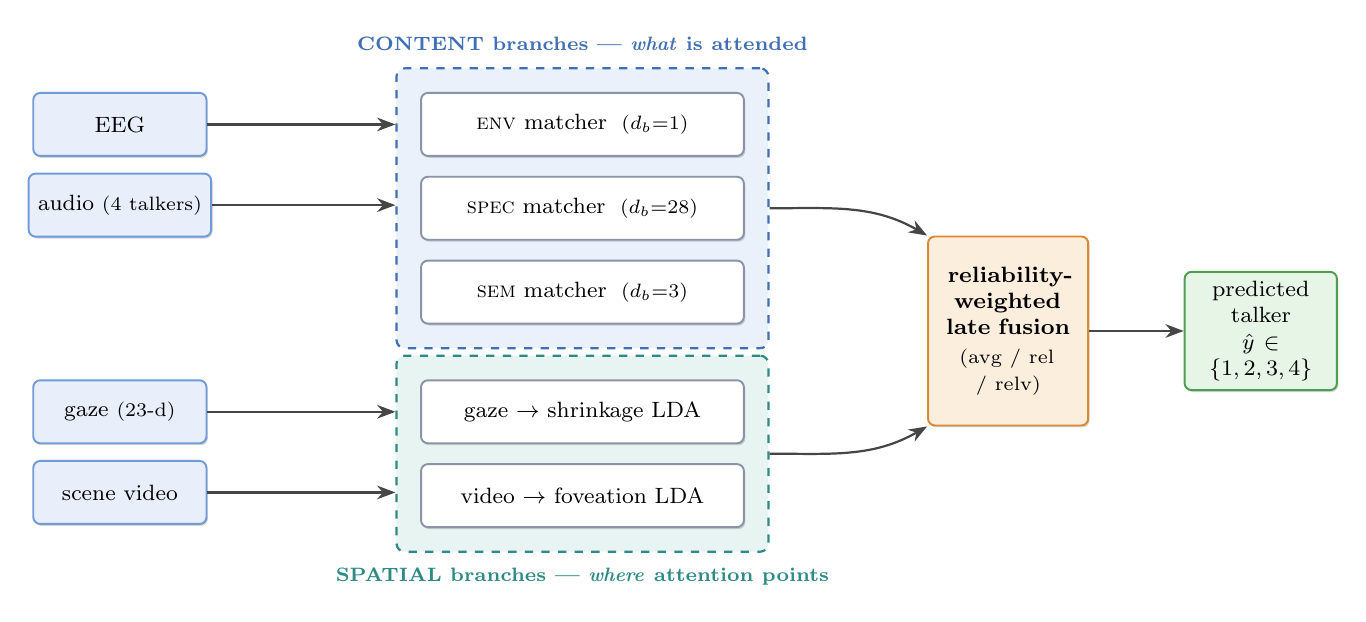
\begin{tikzpicture}[font=\footnotesize]
  % --- inputs ---
  \node[inp,minimum width=22mm,minimum height=8mm] (eeg) {EEG};
  \node[inp,minimum width=22mm,minimum height=8mm,below=2mm of eeg] (aud) {audio \scriptsize($4$ talkers)};
  \node[inp,minimum width=22mm,minimum height=8mm,below=18mm of aud] (gaze) {gaze \scriptsize($23$-d)};
  \node[inp,minimum width=22mm,minimum height=8mm,below=2mm of gaze] (vid) {scene video};
  % --- content branches ---
  \node[brn,minimum width=41mm,minimum height=8mm,right=27mm of eeg] (benv) {\textsc{env} matcher \;\scriptsize($d_b{=}1$)};
  \node[brn,minimum width=41mm,minimum height=8mm,below=2.4mm of benv] (bspec){\textsc{spec} matcher \;\scriptsize($d_b{=}28$)};
  \node[brn,minimum width=41mm,minimum height=8mm,below=2.4mm of bspec](bsem) {\textsc{sem} matcher \;\scriptsize($d_b{=}3$)};
  % --- spatial branches ---
  \node[brn,minimum width=41mm,minimum height=8mm,right=27mm of gaze] (bgaze){gaze $\rightarrow$ shrinkage LDA};
  \node[brn,minimum width=41mm,minimum height=8mm,below=2.4mm of bgaze](bvis) {video $\rightarrow$ foveation LDA};
  % --- group boxes ---
  \begin{scope}[on background layer]
    \node[grp,draw=cConB,fill=cCon,fit=(benv)(bsem),inner sep=3mm] (cbox){};
    \node[grp,draw=cSpaB,fill=cSpa,fit=(bgaze)(bvis),inner sep=3mm] (sbox){};
  \end{scope}
  \node[cConB,font=\bfseries\scriptsize] at ([yshift=3mm]cbox.north) {CONTENT branches --- \emph{what} is attended};
  \node[cSpaB,font=\bfseries\scriptsize] at ([yshift=-3mm]sbox.south) {SPATIAL branches --- \emph{where} attention points};
  % --- fusion + output ---
  \coordinate (mid) at ($(cbox.east)!0.5!(sbox.east)$);
  \node[fuse,text width=18mm,minimum height=24mm,right=20mm of mid] (fuse){\textbf{reliability-}\\\textbf{weighted}\\\textbf{late fusion}\\[1pt]\scriptsize(avg / rel / relv)};
  \node[outn,text width=17mm,minimum height=12mm,right=12mm of fuse] (out){predicted talker\\$\hat{y}\!\in\!\{1,2,3,4\}$};
  % --- arrows: inputs -> boxes (horizontal) ---
  \draw[flow] (eeg.east)  -- (eeg.east -| cbox.west);
  \draw[flow] (aud.east)  -- (aud.east -| cbox.west);
  \draw[flow] (gaze.east) -- (gaze.east -| sbox.west);
  \draw[flow] (vid.east)  -- (vid.east  -| sbox.west);
  % --- boxes -> fusion -> output ---
  \draw[flow] (cbox.east) to[out=0,in=150] (fuse.north west);
  \draw[flow] (sbox.east) to[out=0,in=210] (fuse.south west);
  \draw[flow] (fuse.east) -- (out.west);
\end{tikzpicture}
\caption{\textbf{The decoder.} Each branch outputs a four-class probability over
the talkers; frozen branches are fused by weights set from their out-of-fold
reliability. \emph{Content} branches reconstruct a per-talker audio feature from
EEG and match it to the four candidates (Eq.~\ref{eq:corr}); \emph{spatial}
branches classify where the listener orients, from gaze and (Section
\ref{sec:asd-video}) from video. EEG and audio feed the content family; gaze and
video feed the spatial family. Per-branch layers are in Table~\ref{tab:arch}.}
\label{fig:arch}
\end{figure*}

\subsection{Content branches: is the brain tracking the attended talker?}
\label{sec:asd-content}

\paragraph{The idea, and the two traps we must avoid.}
A content branch reconstructs a feature of the attended speech from EEG and then
asks which of the four talkers that reconstruction best matches. The obvious way
to ``decode the talker''---feed EEG and audio to a classifier---fails honestly
here for two reasons specific to this dataset. \emph{First, loudness.} The
attended talker is mixed louder, so a classifier could read attention off
amplitude alone, telling us nothing about the brain. \emph{Second, clip
identity.} Every subject hears the same clips in the same order, so a network can
memorise which clip is which rather than decode attention. Our matching design
defuses both, as follows.

\paragraph{Matching by correlation defuses loudness.}
The branch maps EEG to a reconstruction $\hat{\mathbf r}\!\in\!\mathbb R^{d_b\times T}$
and scores each candidate $\mathbf c_k$ by their \emph{correlation}, after
z-scoring every candidate per band:
\begin{equation}
s_k=\frac{1}{d_b T}\sum_{d,t}\tilde r_{d,t}\,\tilde c^{\,k}_{d,t},\quad
\tilde x=\frac{x-\bar x}{\sigma_x+\epsilon},\quad z_k=e^{\gamma}s_k .
\label{eq:corr}
\end{equation}
Because correlation is scale-free, loudness cannot help: an uninformative EEG
reconstruction correlates $\approx\!0$ with \emph{every} talker, so the branch
can only win by reconstructing genuine temporal structure. We correlate over the
\emph{whole} $\approx\!30$\,s trial rather than short windows because the
EEG--speech coupling is tiny instant-to-instant; integrating over the trial
accumulates the weak but consistent signal. $\gamma$ is a single learned
temperature ($e^{\gamma}\!\le\!100$) and the branch is trained with cross-entropy
on $\{z_k\}$.

\paragraph{Permuting the candidates defuses clip-identity leakage.}
We drop self-supervised audio embeddings (\textsc{w2v}/HuBERT), which we found
memorise clip identity even after our other controls, and keep only acoustic and
light semantic features. More importantly, on every trial we \emph{shuffle} the
four candidate streams and ask the branch to predict the attended \emph{slot},
not a fixed talker index; the prediction is mapped back to the physical talker
only afterwards. Since the matcher never sees a stable talker$\rightarrow$position
mapping, it cannot exploit position or clip identity---the design is leak-free by
construction, which our null (Section~\ref{sec:asd-results}) then verifies.

\paragraph{What feature to reconstruct, and the encoder that does it.}
We probe three rungs of the speech hierarchy, to see where (if anywhere) EEG
tracks the talker: the broadband \textbf{envelope} (\textsc{env}, $d_b\!=\!1$;
the classic attention correlate), the $28$-band \textbf{spectrogram}
(\textsc{spec}, $d_b\!=\!28$; finer spectro-temporal detail), and a light
\textbf{semantic} embedding (\textsc{sem}, $d_b\!=\!3$). The EEG encoder
(Table~\ref{tab:arch}a) is deliberately shaped to the neuroscience: the cortical
response to speech is smeared across lags from $0$ to $\sim\!400$\,ms with
structure at several timescales, so after a $1{\times}1$ spatial mix we apply
\emph{four temporal convolutions with dilations $1,2,4,8$ in parallel}, giving
receptive fields that span that lag range at low parameter cost, before a
$1{\times}1$ projection to the feature dimension $d_b$.

% ---- full-width architecture table: anchored in the Model section ----
\begin{table*}[t]
\centering
\caption{\textbf{Per-branch architecture.} All convolutions are $1$-D over time
($T\!=\!1908$); hidden width $H\!=\!64$; $d_b$ is the reconstructed feature
dimension. ``k''$=$kernel, ``pad''$=$padding, ``$d$''$=$dilation. Every branch is
frozen before fusion. Panels: (a) the content matcher (\S\ref{sec:asd-content}),
(b,c) the gaze branch heads (\S\ref{sec:asd-spatial}), (d) the MS$+$recon ablation
(\S\ref{sec:asd-results}).}
\label{tab:arch}
\footnotesize
\begin{tabular}{@{}>{\raggedright\arraybackslash}p{0.19\textwidth}>{\raggedright\arraybackslash}p{0.60\textwidth}l@{}}
\toprule
Stage & Configuration & Output \\
\midrule
\multicolumn{3}{@{}l}{\emph{(a) Content matcher} --- dilated EEG encoder $+$ $1{\times}1$ projection $+$ correlation scoring (one per feature)}\\
Input EEG & --- & $32\times T$ \\
Spatial mix & Conv1d $32\!\to\!64$, k$1$ & $64\times T$ \\
Temporal ($\times4$, parallel) & Conv1d $64\!\to\!64$, k$15$, $d\in\{1,2,4,8\}$, pad $7d$, ELU & $4\times(64\times T)$ \\
Concatenate $+$ normalize & BatchNorm, ELU & $256\times T$ \\
Project & Conv1d $256\!\to\!64$, k$1$, Dropout $0.3$ & $64\times T$ \\
Decode & Conv1d $64\!\to\!d_b$, k$1$ & $d_b\times T\ (\hat{\mathbf r})$ \\
Score & correlation vs.\ $4$ candidates, $\times\,e^{\gamma}$ (Eq.~\ref{eq:corr}) & $4$ logits \\
\multicolumn{3}{@{}r}{\footnotesize params $=2.652/2.653/2.669\times10^{5}$ for $d_b=1/3/28$}\\
\midrule
\multicolumn{3}{@{}l}{\emph{(b) Gaze branch, \textsc{mlp} head} --- EEG encoder $+$ gaze MLP (comparison)}\\
Conv blocks $\times3$ & Conv1d (k$25$,k$15$,k$15$), BN, ELU, Drop $0.3$ & $64\times T$ \\
Pool $+$ gaze & mean over $T$, $\oplus\,23$-d gaze & $87$ \\
Head & Linear $87\!\to\!64$, ELU, Drop $0.3$, Linear $64\!\to\!4$ & $4$ logits \\
\multicolumn{3}{@{}r}{\footnotesize params $=1.805\times10^{5}$}\\
\midrule
\multicolumn{3}{@{}l}{\emph{(c) Gaze branch, \textsc{lda} head} --- gaze only (our choice)}\\
Input gaze & per-subject z-scored & $23$ \\
Classifier & LDA, lsqr solver, Ledoit--Wolf shrinkage & $4$ posteriors \\
\multicolumn{3}{@{}r}{\footnotesize closed-form; no SGD; cannot overfit}\\
\midrule
\multicolumn{3}{@{}l}{\emph{(d) MS$+$recon encoder} (content ablation, \S\ref{sec:asd-results}; replaces the encoder in (a))}\\
Encoder & Conv1d $32\!\to\!64$ k$1$, BN, ELU; $\times4$ Conv1d $64\!\to\!64$ k$5$ $d\in\{1,2,4,8\}$ ELU; Drop $0.2$; Conv1d $256\!\to\!d_b$ k$1$ & $d_b\times T$ \\
Aux.\ loss & $\mathrm{MSE}+(1-\mathrm{corr})$ to attended candidate & --- \\
\multicolumn{3}{@{}r}{\footnotesize params $=0.916\times10^{5}$ ($d_b=28$)}\\
\bottomrule
\end{tabular}
\end{table*}

\subsection{Spatial branches: where is the listener looking?}
\label{sec:asd-spatial}

\paragraph{Gaze is the strong cue---but the data are scarce and uncalibrated.}
In a free-field room, listeners often look toward the talker they attend, so
gaze is informative. We summarise it as a $23$-dimensional vector (horizontal and
vertical gaze mean/variance, per-eye azimuth/elevation, saccade rate and
amplitude, pupil size, head-motion magnitude, and signal validity). The
difficulty is statistical: each subject gives only $\sim\!80$ training trials, so
a flexible network that ingests EEG and gaze together \emph{overfits} this tiny
set. Our remedy is to classify the gaze vector with a \emph{shrinkage linear
discriminant} (Ledoit--Wolf): it is closed-form, has no capacity to overfit, and
regularises the class covariances toward a stable estimate---which turned out to
be the single most effective choice in the whole model
(Section~\ref{sec:asd-results}). For comparison we also report an EEG$+$gaze MLP
head (Table~\ref{tab:arch}b,c).

\paragraph{Calibrating gaze across subjects.}
The eye-tracker is uncalibrated and reports \emph{subject-relative} positions.
Within a subject this is harmless. Across subjects (for the LOSO protocol) it is
not: raw values live on different scales, so a pooled classifier would compare
apples to oranges. Before pooling we therefore z-score each gaze feature
\emph{within each subject using only that subject's own trials}---a label-free
standardisation, the minimal calibration the leave-one-subject-out setting
permits.

\paragraph{Fusing branches by reliability, not by vote.}
The branches differ greatly in quality (content $\approx\!0.4$, gaze
$\approx\!0.55$). A plain average would let three weak content branches drown the
strong gaze one, so we weight each branch by how far its \emph{out-of-fold}
accuracy exceeds chance, $w_b\!\propto\!\max(0,\mathrm{acc}^{\text{oof}}_b-0.25)$,
estimated on training data only. We further allow a per-trial \emph{validity
gate} that down-weights gaze on trials where the eye signal is poor
(\textsc{relv}), and compare against a uniform average (\textsc{avg}) and a
learned logistic stacker (\textsc{stack}). All fusion parameters are fit on inner
out-of-fold predictions, never on the test fold.

\FloatBarrier
\subsection{How we train and test}
\label{sec:asd-train}

The learnable branches (content matchers and the MLP head) train with AdamW
(learning rate $10^{-3}$, weight decay $10^{-3}$, batch $48$, $30$ epochs,
cross-entropy with label smoothing $0.05$); the LDA head and the fusion
combiners are closed-form. We test under two protocols. \emph{Within-subject}: a
$5$-fold split over each subject's own trials, trial-disjoint. \emph{Leave-one-
subject-out (LOSO)}: train on $15$ subjects, test on the held-out one, repeated
for all $16$. Fusion weights always come from an inner out-of-fold split of the
training data. Finally, as the decisive honesty check, an \textbf{input-shuffle
null} breaks the pairing between the label and every input (EEG, gaze, video)
while leaving the pipeline intact: a model that decodes anything real must here
fall to chance. Table~\ref{tab:hp} collects all settings.

\begin{table}[H]
\centering
\caption{\textbf{Settings and dimensions}, sufficient to reproduce every number.}
\label{tab:hp}
\small
\begin{tabular}{@{}ll@{}}
\toprule
Item & Value \\
\midrule
EEG channels / rate / length & $32$ / $64$\,Hz / $T{=}1908$ ($\approx\!30$\,s) \\
Reconstructed dim $d_b$ & env $1$, spec $28$, sem $3$ \\
Candidates (permuted) & $4$ attendable talkers \\
Gaze feature dim & $23$ \\
Hidden width / dropout & $64$ / $0.3$ (MS: $0.2$) \\
Corr.\ temperature $\gamma$ & init $2.3$, $e^{\gamma}\!\le\!100$ \\
Optimizer / lr / weight decay & AdamW / $10^{-3}$ / $10^{-3}$ \\
Batch / epochs / label smooth. & $48$ / $30$ / $0.05$ \\
Gaze classifier & LDA, Ledoit--Wolf shrinkage \\
Stacker & logistic, $C{=}0.3$ \\
Reliability weight $w_b$ & $\max(0,\mathrm{acc}^{\mathrm{oof}}_b-0.25)$ \\
\textsc{relv} gate & $w_{\textsc{gaze}}\!\cdot\!\text{validity}$ \\
OOF / within / LOSO splits & $3$-fold / $5$-fold / $16$-fold \\
Seeds (perm.\ / global) & $20260619$ / $0$ \\
\bottomrule
\end{tabular}
\end{table}

\subsection{Results}
\label{sec:asd-results}

Table~\ref{tab:results} reports every accuracy. We read it around three questions:
how strong is each single cue, how much can the brain's \emph{content} signal give
on its own, and how much does overt \emph{orienting} add.

\paragraph{Single cues: content is weak but real, orienting is strong.}
Each content branch sits clearly above its null yet well below the spatial cues
(within-subject \textsc{env}~\intraEnv, \textsc{spec}~\intraSpec,
\textsc{sem}~\intraSem; chance $0.25$): the brain carries a faint but reliable
trace of the attended talker. In this free-field room overt orienting dominates,
as expected---the gaze branch reaches \intraDirLda, and the video branch more
still (Section~\ref{sec:asd-video}).

\paragraph{The honest content number, kept separate from orienting.}
Because content and orienting answer different scientific questions, we report two
\emph{partial} fusions next to the full one (Table~\ref{tab:results}, middle
block). \textbf{Content-only} pools just \textsc{env}/\textsc{spec}/\textsc{sem}
and is the honest EEG-content number; \textbf{orienting} pools the gaze and video
branches (an overt-behaviour number). Content-only fuses to
\pmv{\cfusedI}{\cfusedIS}---real, but modest---whereas orienting reaches
\pmv{\sfusedI}{\sfusedIS} from gaze alone; the full model combines both to
\intraLdaRel. Reporting the split keeps the strong orienting cue from being
mistaken for content decoding.

\paragraph{The winning lever is regularisation, not capacity.}
Our largest single gain comes from replacing the EEG$+$gaze \textbf{MLP} head
(\intraDirMlp) with the closed-form \textbf{LDA} head (\intraDirLda): with only
$\sim\!80$ trials per subject the MLP overfits the gaze cue, and the shrinkage
estimator does not. Through fusion this lifts the no-video accuracy from
\intraMlpRel\ (best MLP-head fusion) to \intraLdaRelv\ (\textsc{lda}$+$\textsc{relv}).
Two ``smarter'' ideas instead \emph{backfire}, for the same small-data reason: a
learned logistic stacker underperforms a plain average (\intraMlpStack\ vs.\
\intraMlpAvg), and adding a reconstruction auxiliary on a multi-scale encoder
(Table~\ref{tab:arch}d) pushes content toward chance
(\msrEnv/\msrSpec/\msrSem) despite using \emph{fewer} parameters---the auxiliary
objective competes with the discriminative one. The benefit is concentrated in
subjects who actually move their eyes (individuals $0.87\!\to\!0.94$,
$0.84\!\to\!0.93$); those who stay still sit near chance in every gaze decoder---a
limit of behaviour, not of the model.

\paragraph{Cross-subject (LOSO) and the null.}
Accuracy drops as expected (Table~\ref{tab:results}, right): content-only falls to
\pmv{\losoCfused}{\losoCfusedS} and gaze to \losoDirLda. Yet the video branch
still generalises (\pmv{\losoVisFov}{\losoVisFovS}) and lifts the full model from
\losoLdaRel\ without video to \textbf{\losoFusedVid}. Under the input-shuffle null
the pipeline collapses to chance in both protocols
(\pmv{\nullFused}{\nullFusedS} within; \pmv{\nullLosoFused}{\nullLosoFusedS} LOSO),
confirming nothing leaks.

\begin{table}[H]
\centering
\caption{\textbf{Attended-speaker accuracy} (four-class, chance $0.25$;
mean$\pm$s.d.\ over $16$ subjects). \emph{Within}$=$within-subject $5$-fold;
\emph{LOSO}$=$leave-one-subject-out. \emph{Content-only}
and \emph{orienting} are partial fusions of the content branches and the spatial
branches respectively; \emph{full} fuses all branches. \textbf{Bold}$=$best full
fusion per protocol. Video rows: Section~\ref{sec:asd-video}.}
\label{tab:results}
\small
\setlength{\tabcolsep}{4.5pt}
\begin{tabular}{@{}l r r@{}}
\toprule
Cue / fusion & Within & LOSO \\
\midrule
\multicolumn{3}{@{}l}{\emph{Single-cue branches}}\\
\quad Envelope \footnotesize(content)            & \acc{\intraEnv}{\intraEnvS}   & \acc{\losoEnv}{\losoEnvS} \\
\quad Spectrogram \footnotesize(content)         & \acc{\intraSpec}{\intraSpecS} & \acc{\losoSpec}{\losoSpecS} \\
\quad Semantic \footnotesize(content)            & \acc{\intraSem}{\intraSemS}   & \acc{\losoSem}{\losoSemS} \\
\quad Gaze, \textsc{mlp} \footnotesize(spatial)  & \acc{\intraDirMlp}{\intraDirMlpS} & \acc{\losoDirMlp}{\losoDirMlpS} \\
\quad Gaze, \textsc{lda} \footnotesize(spatial)  & \acc{\intraDirLda}{\intraDirLdaS} & \acc{\losoDirLda}{\losoDirLdaS} \\
\quad Video, scene$+$fovea \footnotesize(spatial)& \acc{\visSF}{\visSFS}         & \acc{\losoVisSF}{\losoVisSFS} \\
\quad Video, \textbf{fovea-only} \footnotesize(spatial)& \acc{\visFov}{\visFovS} & \acc{\losoVisFov}{\losoVisFovS} \\
\midrule
\multicolumn{3}{@{}l}{\emph{Fused decisions}}\\
\quad Content only \footnotesize(env/spec/sem)   & \acc{\cfusedI}{\cfusedIS}     & \acc{\losoCfused}{\losoCfusedS} \\
\quad Orienting \footnotesize(gaze)              & \acc{\sfusedI}{\sfusedIS}     & \acc{\losoSfusedGaze}{\losoSfusedGazeS} \\
\quad Orienting \footnotesize(gaze$+$video)      & \acc{\sfusedVid}{\sfusedVidS} & \acc{\losoSfusedVid}{\losoSfusedVidS} \\
\quad Full, no video                             & \acc{\intraLdaRel}{\intraLdaRelS} & \acc{\losoLdaRel}{\losoLdaRelS} \\
\quad Full, $+$ video \footnotesize(rel)         & \acc{\fusedFovRel}{\fusedFovRelS} & \acc{\losoFusedVid}{\losoFusedVidS} \\
\quad Full, $+$ video \footnotesize(relv)        & \textbf{\acc{\fusedFovRelv}{\fusedFovRelvS}} & \textbf{\acc{\losoFusedRelv}{\losoFusedRelvS}} \\
\midrule
Null, full model        & \acc{\nullFused}{\nullFusedS}   & \acc{\nullLosoFused}{\nullLosoFusedS} \\
Null, content-only      & \acc{\nullCfused}{\nullCfusedS} & \acc{\losoNullCfused}{\losoNullCfusedS} \\
\bottomrule
\end{tabular}
\end{table}

\subsection{Adding vision: what does the scene video buy us?}
\label{sec:asd-video}

\paragraph{Why ordinary ``video for speech'' does not apply here.}
It is tempting to reach for lip-reading or audio--visual speech separation. But
those methods read \emph{faces}, and our scene video has none: it looks out at a
room of loudspeakers (Fig.~\ref{fig:inputs}, bottom-right). Nothing in the pixels
tracks speech content. The one thing the video genuinely adds is \emph{room-frame
orientation}---which loudspeaker the listener is looking at---and, conveniently,
the glasses report gaze in scene-camera pixels, so we can crop a foveal patch
around the gaze point \emph{without any calibration}. We therefore test two
separate questions: \textbf{(i)} does a video ``where'' cue beat the gaze branch,
and \textbf{(ii)} can the video help the EEG content branches, by teaching their
encoder during training? Figure~\ref{fig:vidarch} shows both paths.

\begin{figure*}[t]
\centering
\begin{tikzpicture}[font=\footnotesize,
  thumb/.style={draw=gray!55,line width=0.5pt,inner sep=1pt},
  lbl/.style={font=\scriptsize,gray!45!black}]
  % --- input thumbnails (real frames) ---
  \node[thumb] (scene) {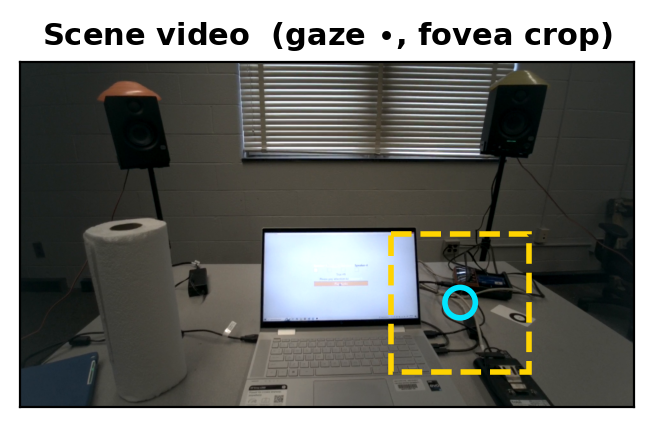
\includegraphics[width=17mm]{ico_scene.png}};
  \node[thumb,below=11mm of scene] (fov) {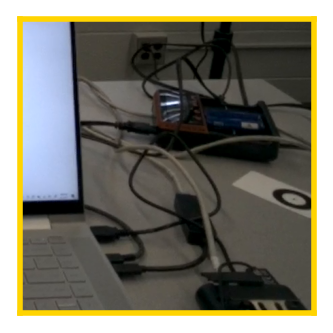
\includegraphics[width=12mm]{ico_fovea.png}};
  \node[lbl,below=0.3mm of scene.south,anchor=north] {scene clip};
  \node[lbl,below=0.3mm of fov.south,anchor=north] {fovea clip};
  % --- frozen encoder, centred between the two thumbnails ---
  \coordinate (vc) at ($(scene.east)!0.5!(fov.east)$);
  \node[frz,text width=20mm,minimum height=14mm] (vjepa) at ([xshift=28mm]vc)
       {\textbf{Frozen}\\\textbf{V-JEPA\,2} ViT-L\\\scriptsize mean-pool};
  % --- two embeddings: fovea (used) on top, scene (near-constant) below ---
  \node[emb,text width=15mm,minimum height=8mm,above right=4mm and 9mm of vjepa] (femb)
       {\textbf{fovea} $1024$};
  \node[emb,text width=18mm,minimum height=8mm,below right=4mm and 9mm of vjepa] (semb)
       {scene $1024$\\\scriptsize\itshape near-constant};
  % --- TEST path: fovea -> vision branch -> p_vis -> fusion -> output ---
  \node[vbr,text width=22mm,minimum height=11mm,right=8mm of femb] (vbr)
       {\textbf{vision branch}\\PCA $\to$ shrinkage LDA};
  \node[emb,text width=10mm,minimum height=8mm,right=7mm of vbr] (pvis) {$\mathbf p^{(\textsc{vis})}$};
  \node[fuse,text width=14mm,minimum height=12mm,right=8mm of pvis] (fuse)
       {\textbf{late}\\\textbf{fusion}};
  \node[outn,text width=15mm,minimum height=12mm,right=7mm of fuse] (out)
       {predicted talker $\hat y$};
  \node[ghost,text width=22mm,minimum height=8mm,above=6mm of fuse]
       (ghost) {content $+$ gaze\\posteriors (Fig.~\ref{fig:arch})};
  % --- TRAIN-ONLY alignment block: scene emb is the target ---
  \node[frz,text width=16mm,minimum height=9mm,below=12mm of semb] (proj) {project $P_\phi$};
  \node[brn,text width=18mm,minimum height=9mm,left=15mm of proj] (eegc)
       {EEG content\\recon.\ $\bar{\mathbf r}$};
  \begin{scope}[on background layer]
    \node[grp,draw=cFusB,fill=cFus!55,fit=(eegc)(proj),inner sep=3mm] (tbox){};
  \end{scope}
  \node[cFusB,font=\bfseries\scriptsize] at ([yshift=-2.8mm]tbox.south)
       {train-time only --- removed at test};
  % --- solid: test/inference path (fovea only) ---
  \draw[flow](scene.east)--(vjepa.west);
  \draw[flow](fov.east)--(vjepa.west);
  \draw[flow](vjepa)--(femb);
  \draw[flow](vjepa)--(semb);
  \draw[flow](femb)--(vbr);
  \draw[flow](vbr)--(pvis);
  \draw[flow](pvis)--(fuse);
  \draw[flow](ghost)--(fuse);
  \draw[flow](fuse)--(out);
  % --- dashed: scene -> train-only alignment ---
  \draw[flowd](semb.south)--(proj.north) node[midway,right,font=\scriptsize]{target};
  \draw[<->,line width=0.8pt,dashed,cFusB] (eegc)--(proj)
       node[midway,above,font=\scriptsize,text=cFusB]{InfoNCE};
\end{tikzpicture}
\caption{\textbf{Video path, and how it plugs into the model.} A frozen
V-JEPA\,2 encoder maps each trial's \emph{scene} clip and gaze-centred
\emph{fovea} clip to a $1024$-d vector each. \textbf{Test path (solid):} only the
\emph{fovea} embedding feeds the vision branch (PCA $\to$ shrinkage LDA) $\to$
posterior $\mathbf p^{(\textsc{vis})}$, which enters the \emph{same}
reliability-weighted late fusion as the content and gaze branches of
Fig.~\ref{fig:arch} to give the predicted talker $\hat y$. The \emph{scene}
embedding is near-constant across trials---the camera barely moves in this
room---so it is dropped from the branch (the ``fovea-only'' setting that wins in
Table~\ref{tab:results}). \textbf{Train-only path (dashed):} that scene embedding
instead serves as the \emph{target} of an InfoNCE alignment (Eq.~\ref{eq:infonce})
on the EEG content reconstruction $\bar{\mathbf r}$; this block is removed at test,
so video never touches inference for content.}
\label{fig:vidarch}
\end{figure*}

\paragraph{One frozen video encoder, used two ways.}
We never train on pixels---$16$ subjects is far too little to fit a video model,
and it would simply memorise the room. Instead we run a \emph{frozen},
self-supervised V-JEPA\,2 encoder (ViT-L) over $64$ frames sampled across each
trial's \emph{audio window} (so the video is time-aligned to the listening task),
in two forms: a full-frame \emph{scene} clip and a gaze-centred \emph{fovea} clip
($256^2$ crop), each mean-pooled to a $1024$-d embedding
(Table~\ref{tab:vidarch}a). This costs one offline pass ($\approx\!8$\,min/subject).

\paragraph{(i) The vision branch.}
To answer ``does video beat gaze'', we add a spatial branch that classifies the
video embedding $\mathbf v$ into the four talkers. As with gaze, $\sim\!1000$
dimensions over $\sim\!80$ trials demand strong regularisation, so we standardise,
reduce by PCA ($\le\!24$ components), and use the same shrinkage LDA:
\begin{equation}
\mathbf u=W_{\text{pca}}^{\!\top}\frac{\mathbf v-\boldsymbol\mu}{\boldsymbol\sigma},
\qquad
\mathbf p^{(\textsc{vis})}=\mathrm{LDA}_{\text{LW}}(\mathbf u)\in\Delta^3,
\label{eq:vis}
\end{equation}
fit on the training fold only (per-subject standardisation for LOSO, as for gaze);
no video weights are gradient-trained. We use the \emph{fovea} embedding alone
($\mathbf v\!=\!\mathbf v_{\text{fovea}}\!\in\!\mathbb R^{1024}$): the scene view
barely changes across trials, so its embedding is near-constant and only adds
noise---concatenating it ($\mathbf v\!\in\!\mathbb R^{2048}$) is the weaker
ablation in Table~\ref{tab:results}. The scene embedding is instead put to use as
the \emph{alignment target} below.

\paragraph{(ii) Teaching the EEG encoder with video.}
To answer ``can video help content'', we add a \emph{training-only} loss that
pulls a content branch's pooled reconstruction
$\bar{\mathbf r}_i\!=\!\tfrac1T\sum_t\mathbf r_{i,:,t}$ toward the trial's scene
embedding $\mathbf s_i$. The hope is that ``where the listener looks'' nudges the
EEG encoder toward attention-relevant structure. We learn a projection
$P_\phi\!:\!\mathbb R^{1024}\!\to\!\mathbb R^{d_b}$, normalise both sides, and use
a within-batch InfoNCE that makes each trial's EEG match \emph{its own} video
against the other trials in the batch:
\begin{equation}
\mathbf a_i=\tfrac{\bar{\mathbf r}_i}{\lVert\bar{\mathbf r}_i\rVert},\;
\mathbf b_i=\tfrac{P_\phi\mathbf s_i}{\lVert P_\phi\mathbf s_i\rVert},\;
\label{eq:alignembed}
\end{equation}
\begin{equation}
\mathcal L_{\text{align}}=-\frac{1}{2|\mathcal B|}\!\sum_{i\in\mathcal B}\!\Bigg[
\log\frac{e^{\mathbf a_i^{\!\top}\mathbf b_i/\tau}}{\sum_je^{\mathbf a_i^{\!\top}\mathbf b_j/\tau}}
+\log\frac{e^{\mathbf a_i^{\!\top}\mathbf b_i/\tau}}{\sum_je^{\mathbf a_j^{\!\top}\mathbf b_i/\tau}}\Bigg],
\label{eq:infonce}
\end{equation}
added to the usual objective,
$\mathcal L=\mathcal L_{\text{CE}}+\lambda_{\text{rec}}\mathcal L_{\text{rec}}
+\lambda_{\text{align}}\mathcal L_{\text{align}}$
($\tau\!=\!0.1$, $\lambda_{\text{align}}\!=\!0.3$). Video enters \emph{only} here
and is dropped at test. Crucially, this loss requires the alternative MS$+$recon
encoder, which by itself changes content accuracy; so we also run that encoder
\emph{with the alignment switched off} ($\lambda_{\text{align}}\!=\!0$), as a
control that separates ``the encoder'' from ``the video''.

\begin{table}[H]
\centering
\caption{\textbf{Video-path stages.} The encoder is frozen; the vision branch (b)
is closed-form; only the alignment head (c) is learned, and only during training.}
\label{tab:vidarch}
\small
\begin{tabular}{@{}>{\raggedright\arraybackslash}p{0.62\columnwidth}r@{}}
\toprule
Stage & Output \\
\midrule
\multicolumn{2}{@{}l}{\emph{(a) Frozen features (per clip)}}\\
Input clip ($64$ frames, audio window) & $64\!\times\!3\!\times\!256^2$ \\
V-JEPA\,2 ViT-L (frozen), mean-pool & $1024$ \\
$\to$ fovea emb / scene emb & $1024$ each \\
\midrule
\multicolumn{2}{@{}l}{\emph{(b) Vision branch (closed-form; \textbf{fovea} only)}}\\
Standardise (train fold) $+$ PCA & $\le\!24$ \\
Shrinkage LDA & $4$ posteriors \\
\midrule
\multicolumn{2}{@{}l}{\emph{(c) Alignment head (train only; \textbf{scene} target)}}\\
$P_\phi:\mathbb R^{1024}\!\to\!\mathbb R^{d_b}$; InfoNCE & scalar \\
\multicolumn{2}{@{}r}{\footnotesize learned params $=1024\,d_b$ ($\approx\!29$k, \textsc{spec})}\\
\bottomrule
\end{tabular}
\end{table}

\paragraph{(i) Result: video is the strongest cue, and fovea-only wins.}
The fovea vision branch reaches \pmv{\visFov}{\visFovS} within subject, beating
gaze (\intraDirLda) and every content branch, with the largest fusion weight
($w_{\textsc{vis}}\!=\!\visWeight$). Using the fovea crop \emph{alone} beats
concatenating it with the full-scene embedding (\visFov\ vs.\ \visSF), confirming
the scene half is near-constant noise. Folding the fovea branch in raises the
orienting fusion from \pmv{\sfusedI}{\sfusedIS} (gaze only) to
\pmv{\sfusedVid}{\sfusedVidS}, and the full model from \intraLdaRel\ to
\textbf{\fusedFovRel} (\textsc{rel}) / \textbf{\fusedFovRelv} (\textsc{relv}),
about $+0.08$; the gain transfers to LOSO (branch
\pmv{\losoVisFov}{\losoVisFovS}, full \textbf{\losoFusedVid} vs.\ \losoLdaRel\
without video). But this is still \emph{where}, not \emph{what}: the branch reads
which loudspeaker is foveated, so we count it with the orienting cues, and the
honest content number (content-only fusion) is unchanged at \cfusedI.

\paragraph{(ii) Result: video does \emph{not} help content.}
The training-time alignment is inert (Table~\ref{tab:content}). Turning it on
leaves the content branches where the MS$+$recon encoder \emph{without} alignment
already puts them---content-only fusion \pmv{\cfusedVal}{\cfusedValS}, statistically
the content null---and this holds for \emph{both} a scene target and a fovea
target. The drop from the original encoder is thus the \emph{encoder swap}, not the
video. The whole pipeline passes the null too: with every input unpaired it
collapses to chance (full \pmv{\nullFused}{\nullFusedS}, content-only
\pmv{\nullCfused}{\nullCfusedS}, vision branch \pmv{\nullVis}{\nullVisS}).
\textbf{In sum, video adds a strong spatial cue but makes the brain's content
signal no more decodable on this corpus.}

\begin{table}[H]
\centering
\caption{\textbf{Video does not help content.} Content-branch accuracy
(within-subject, chance $0.25$). Swapping in the MS$+$recon encoder lowers content;
adding the video-alignment loss \emph{on top}---with either a scene or a fovea
target---changes nothing. The loss is inert; the drop is the encoder, not the video.}
\label{tab:content}
\small
\setlength{\tabcolsep}{6pt}
\begin{tabular}{@{}l r r r@{}}
\toprule
Encoder / objective & \textsc{env} & \textsc{spec} & \textsc{sem} \\
\midrule
Original encoder \footnotesize(baseline) & $\intraEnv$ & $\intraSpec$ & $\intraSem$ \\
MS$+$recon \footnotesize(control, no align) & $\msrEnv$ & $\msrSpec$ & $\msrSem$ \\
\quad $+$ video align, scene target      & $\valEnv$   & $\valSpec$   & $\valSem$ \\
\quad $+$ video align, fovea target      & $\valfEnv$  & $\valfSpec$  & $\valfSem$ \\
\bottomrule
\end{tabular}
\end{table}

\end{document}
